\documentclass[../main.tex]{subfiles}

\begin{document}

\section{Anodes}
\label{sec:anodes}

\subsection{Introduction}
\label{sec:anodes_intro}
Critical to the success of lithium-ion batteries (LiBs) was the development of graphite-based anodes. Graphite proved to be ideal for this application, due to its low (de)-intercalation potential, only slightly higher than that of metallic lithium, and high theoretical gravimetric capacity of 372 mAh g$^{-1}$. However, many key degradation mechanisms in present-day LiBs that lead to their eventual failure, including cracking/reformation of the solid-electrolyte interphase (SEI) and lithium plating, are still intimately connected with graphite-based anodes \cite{VETTER2005269,ma6041310}. The understanding of these mechanisms is still far from complete and leads to complex, non-linear degradation behaviour that is difficult to predict,\cite{YANG201728} motivating the development of multiscale models with a descriptive and predictive capability. A critical starting point for these models is a physically accurate atomistic description of the graphite and its interface with organic electrolytes.

The possibility to form Li-graphite intercalation compounds (Li-GICs), also known as ``stages'', up to a stoichiometry of LiC$_{6}$, was known in 1975, albeit at that time it was only possible to form them by heat treating powders\cite{GUERARD1975337,Woo1983,BASU1979275}. Initial attempts to electrochemically intercalate lithium into graphite resulted in co-intercalation of the organic solvent and exfoliation of the graphite \cite{besenhard1976electrochemical}. In 1983, \citeauthor{yazami1983} reported the first successful intercalation into graphite using a solid polymer electrolyte \cite{yazami1983}. \citeauthor{Fong1990} found that reversible lithium intercalation could be achieved in liquid organic electrolytes using ethylene carbonate (EC) as part of the solvent, which finally enabled the formation of a stable SEI on the graphite surface \cite{Fong1990}. Mixtures of EC and dimethyl carbonate (DMC) were developed by \citeauthor{TARASCON19931221} in 1993 \cite{TARASCON19931221} and present-day graphite-based LiBs are still primarily based on this electrolyte mixture. The key challenge was finding a solvent chemistry that provided sufficient ionic conductivity, did not decompose significantly at the $\sim$4 V cathode potential, while also avoiding co-intercalation into the graphite and producing a stable SEI on its surface. Further incremental improvements in performance have since been achieved through additional additives and, more recently, the inclusion of small amounts of silicon in the anode as a secondary material. 

This section predominantly focuses on graphite, since it remains the primary anode electrode material in the majority of commercial lithium ion (Li-ion) cells \cite{asenbauer_success_2020}. 
Here, the experimentally confirmed Li-graphite stages and the nomenclature necessary for atomistic models of bulk behaviour are defined. Atomistic modelling in the graphite bulk is outlined, including both thermodynamic and kinetic properties. The key graphite surfaces relevant to understanding the initial intercalation are described, then moving to modelling at the graphite edges and the interface with the electrolyte. Throughout, it is shown how these models enable quantitative understanding of the physical mechanisms of Li intercalation in the graphite bulk, the initial insertion at the graphite edges, and the interface between graphite and the electrolyte. Along the way, the key experimentally observable parameters are outlined, showing success stories of atomistic models to not only quantify and describe those parameters but to also predict new behaviour. In some cases, quantitative disagreement between model and experimental observations is also informative and can create new research directions. Work linking atomistic and continuum models is presented in the case of the technologically important SEI. Given the emerging importance of C/Si and C/SiO$_x$ composites in commercial anode materials, some of the challenges in atomistic modelling of Si and related materials are summarised at the end. In the outlook, key remaining challenges are presented for modelling not only graphite, but also next generation materials such as silicides. Challenges related to metallic Li formation on graphite anodes, and the use of metallic Li as an anode material, are also summarised in the outlook.  

\subsection{Bulk Properties}
\label{sec:anode_bulk}
% Mike + incorporated parts from Rana.

\subsubsection{Graphite structure and Li-graphite stages}
\label{sec:anodes_structure_stages}

Graphite possesses a layered structure with carbon atoms forming a network of hexagons in each layer. The carbon atoms located within one layer are covalently bonded to each other, whereas the weak interlayer binding arises from the dispersion or van der Waals (vdW) interactions \cite{GUERARD1975337,Woo1983,persson2010,Woo1983,Dahn1991,hazrati_li_2014,Konar2015}. The lowest energy stacking of the carbon layers is AB stacked (Figure~\ref{fig:graphite_stages_schematics}b), but synthesised graphite structures also contain a small amount of rhombohedral (ABC-stacked) domains \cite{Shi_1996}. 

Li-graphite stages, also known as lithium-graphite intercalation compounds (Li-GICs), are lithium concentration-dependent structures of various stoichiometries \cite{Woo1983,GUERARD1975337,Konar2015,Sethuraman2010,Dahn1991}. In Li-GICs, Li atoms form a 2D hexagonal ($\sqrt{3} \times \sqrt{3}$)R 30 $^{\circ}$ superstructure, with Li atoms sitting directly above each other, as shown in Figure~\ref{fig:graphite_stages_schematics}a. The stage number, $n$, denotes the number of graphene layers between each lithium-filled layer \cite{Dahn1991,Ohzuku1993,Konar2015,GUERARD1975337}.
The experimentally confirmed stages adopt different stackings in the carbon host lattice, as shown in Figure~\ref{fig:graphite_stages_schematics}. The standard nomenclature for GICs \cite{Woo1983} denotes the carbon stacking and Li occupancies: periodic carbon layer stackings along the [001] axis are designated by uppercase letters separated by Greek lowercase letters, if Li is intercalated between planes. For instance, fully lithiated Stage I LiC$_{6}$ ($x=1$) adopts A$\alpha$A$\alpha$A$\alpha$ stacking \cite{Konar2015,He_2013,Yazami_2006}. Here $\alpha$ denotes a lithium filled layer and $x$ is the fraction of Li in Li$_{x}$C$_{6}$ ($0 \leq x \leq 1$).

\begin{figure}[h!]
    \begin{center}
    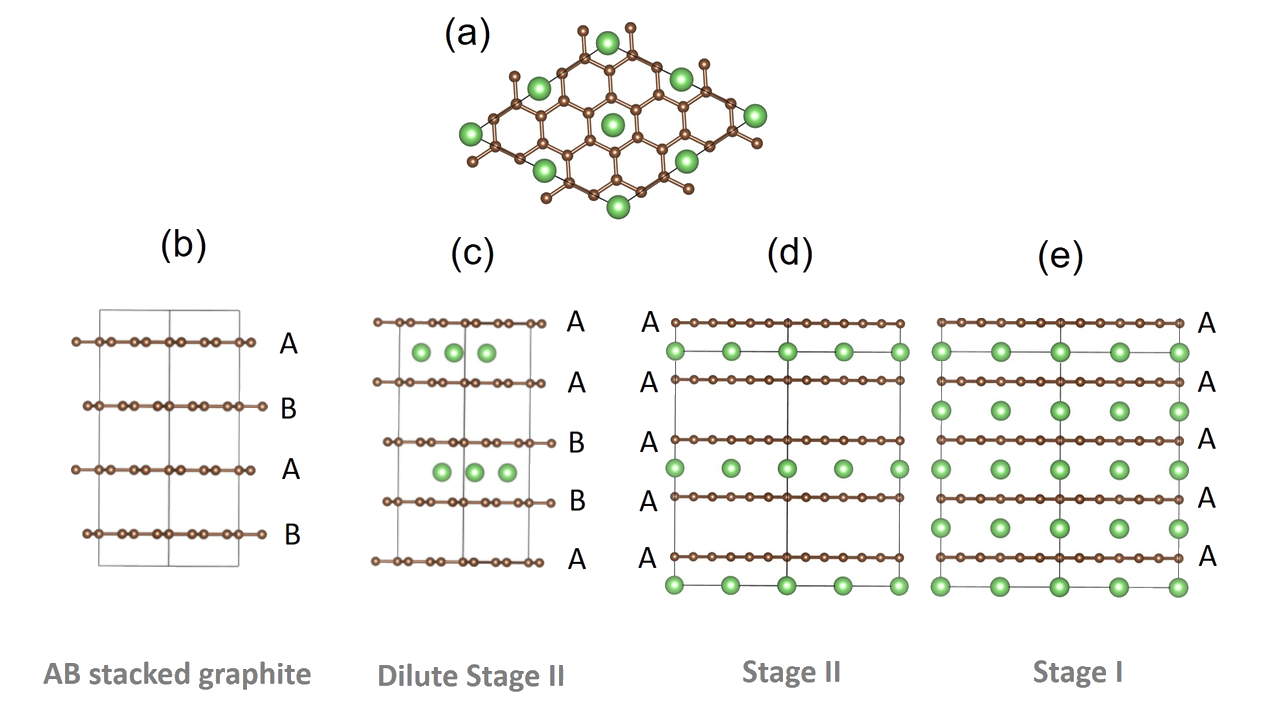
\includegraphics[width=0.98\columnwidth]{figures/stages_version4.png}
    \caption{Structural representations of different carbon stackings in experimentally confirmed stages of graphite. (a) Top down view of carbon and lithium arrangements in Stages I and II. (b-e): side views, showing the layers occupied with Li and carbon stackings in (b) empty AB stacked graphite, (c)~A\(\alpha\)AB\(\beta\)B stacked dilute Stage II, with~\(\beta\) indicating a lithium layer translated with respect to~\(\alpha\), (d)
    A\(\alpha\)AA\(\alpha\)A Stage II and (e)~ A\(\alpha\) stacked Stage I. Green represent Li atoms, while the brown indicate C atoms. Reproduced from Ref.~\citenum{Mercer2021} - Published by The Royal Society of Chemistry.}
    \label{fig:graphite_stages_schematics}
    \end{center}
\end{figure}

Li-GICs vary not only in their lithium concentrations, but also in their carbon stackings. The current consensus of all known stages, including their carbon stackings and lithium stoichiometries, is tabulated in Table~\ref{table:graphite_stages}.

\begin{table}
    \caption{{Overview of carbon stackings and stoichiometries of Li-graphite stages from the literature, where Latin characters denote carbon stackings and Greek characters denote Li-filled layers. \cite{TRUCANO1975,Okamoto1989,GUERARD1975337,Billaud1996,BILLAUD2002299,Woo1983,Dahn1991,Ohzuku1993,Konar2015,didier2020}}}
    \label{table:graphite_stages}
    \begin{tabular}{|c c c|} 
         \hline
         Stage & Stacking & $x$ in Li$_{x}$C$_{6}$  \\
         \hline
         Stage I & A$\alpha$A$\alpha$ & $x = 1$ (LiC$_{6}$)    \\
         Stage II & A$\alpha$AA$\alpha$A & $x = 0.5$ (LiC$_{12}$)  \\
         Dilute Stage II (IID) & A$\alpha$AB$\beta$B & $x \approx 0.33$ (LiC$_{18}$)   \\
         Stage III & A$\alpha$AB/A$\alpha$ABA$\alpha$AC & $x \approx 0.22$ (LiC$_{27}$) \\
         Stage IV & Unknown & $x \approx 0.17$ (LiC$_{36}$)  \\
         Dilute Stage I (ID) & AB & $x \approx 0.083$ (LiC$_{72}$)  \\
         Graphite & AB & $x = 0$   \\
         \hline
    \end{tabular}
\end{table}

Experimental observation of these stages relies largely on probing the average interlayer carbon spacing through diffraction measurements. Probing the lithium orderings of Li-GICs through experimental techniques remains very difficult,\cite{Zheng1995,Konar2015,Senyshyn2013,Taminato2016,Mercer2019,Mercer2021} but as shown in section~\ref{sec:anodes_entropy}, atomistic techniques shed light on these orderings.

Thermodynamic and kinetic properties of Li-GICs have been studied by considering various structures of LiC$_{6n}$ using Density Functional Theory (DFT) \cite{thinius2014theoretical, Hakim, Qiong, Doreen,JI201866,Wang,persson2010,persson2010lithium,hazrati_li_2014,peng2020lithium,hazrati_li_2014}, mean field \cite{Mercer2019,Leiva2017b,OTERO2017569}, canonical and grand canonical Monte Carlo (MC), \cite{Gavil_n_Arriazu_2018,persson2010,C7CP04253A}, and kinetic Monte Carlo (kMC) simulation techniques \cite{JI201866,persson2010,gavilan-arriazu_effect_2020,gavilan-arriazu_kinetic_2020,GAVILANARRIAZU2018133}. The rest of the section outlines electronic structure based studies of experimentally measurable bulk thermodynamic properties, before describing atomistic modelling of kinetic properties.

\subsubsection{Equilibrium potential and measured open circuit voltage}
\label{sec:anodes_ocv}

Knowledge of the correct phase behaviour of an intercalation electrode is an important pre-requisite to building a dynamic model of the intercalation process. One of the most directly measurable observables is the experimental open circuit voltage (OCV), which is related to the equilibrium potential determinable from atomistic methods (c.f. Methods section~\ref{sec:properties_equilibriumvoltage}). The OCV is an important input parameter in continuum models and is also used in control models, for example, to determine the state of charge of a battery within a Battery Management System (BMS) \cite{PLETT2004262}. Inputting a polynomial fit to the experimental OCV at an arbitrary temperature without physical meaning could lead to incorrect predictions of temperature-dependent behaviour in these models. Therefore, to attain predictive, dynamic models on longer length scales, atomistic models of the OCV and equilibrium potential are important and can contribute to physically more robust and more predictive temperature dependence in continuum and control models.\cite{VanderVen2020,Urban2016}

In any intercalation electrode, ordered phases give rise to steps in the OCV. In the lithium-graphite system, the ordered stages described in section~\ref{sec:anodes_structure_stages} therefore give rise to characteristic features in OCV versus $x$ curves \cite{Dahn1991,Ohzuku1993} as shown in Figure~\ref{fig:expt_ocv}.  The influence of the Li-graphite stages on the measured OCV at $T \approx 25$ $^{\circ}$C has been well characterised \cite{Sole2014,Zheng1995,Senyshyn2013,Taminato2016,Allart2018,Sethuraman2010,Markevich2005,Dahn1991,Ohzuku1993}, although a more thorough study of the temperature dependence of the OCV has only been conducted more recently \cite{Mercer2021}. Each OCV plateau represents a different two-phase equilibrium. At zero Kelvin, there is no contribution from configurational entropy and each step represents a sudden transition between two different two-phase equilibria. This is the behaviour that can be captured using DFT code. The cluster expansion framework, described in more detail in the Methods section~\ref{sec:cluster_expansion}, allows the accuracy of DFT to be retained to explore configurational degrees of freedom. Thermal fluctuations can be included by determining effective cluster interactions (ECIs) from fitting DFT data and using these as parameters within an MC method (section~\ref{sec:monte_carlo}). The entropy contribution at temperature, $T > 0$ K has the effect of smoothing out those steps \cite{Mercer2019,OTERO2017569,REYNIER2003850,Mercer2021}, which is caused by some limited single phase solubility around the stoichiometric composition. This can be seen in experimentally measured OCV profiles at $T \approx 300$ K, such as the ones shown in Figure~\ref{fig:expt_ocv}.

\begin{figure}
    \centering
    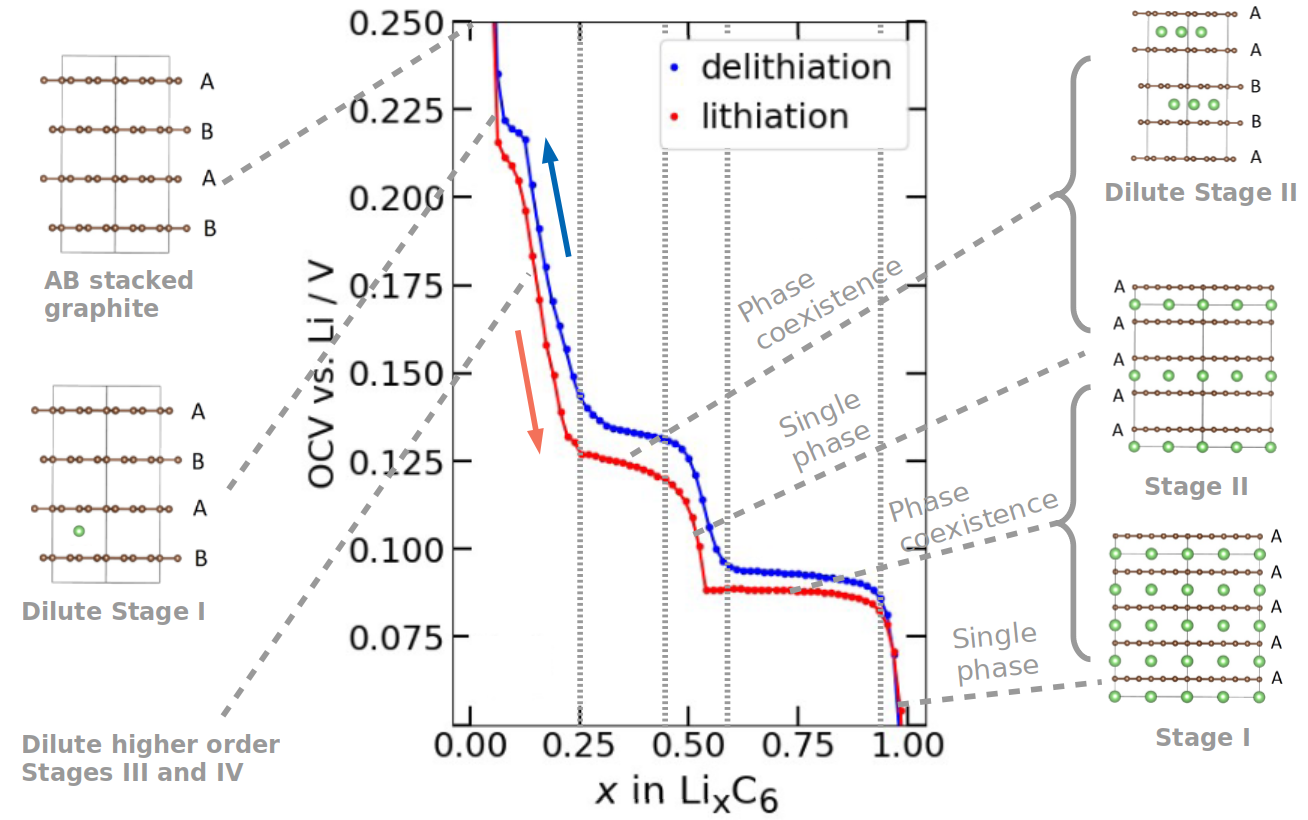
\includegraphics[scale=1.2]{figures/ocv_and_stages.png}
    \caption{Illustration of OCV features of lithium in graphite using experimental data from ref.~\citenum{Mercer2019}. Lithiation and delithiation behaviour is overlaid; labelled stages are linked to the lithiation profile, which is closer to the true equilibrium potential. Reproduced from Ref.~\citenum{Mercer2021} - Published by The Royal Society of Chemistry.}
    \label{fig:expt_ocv}
\end{figure}

The equilibrium potential versus $x$ can be modelled through atomistic techniques. For example, Li-graphite phase diagrams were constructed and the equilibrium potential was modelled by \citeauthor{persson2010} \cite{persson2010}. They performed a cluster expansion of Li degrees of freedom from total energy DFT calculations, by fixing the carbon stacking degrees of freedom. Those degrees of freedom represent the host lattice stackings in the experimentally confirmed stages shown in Figure~\ref{fig:graphite_stages_schematics}. Typically, different cluster expansions are performed in Li-vacancy lattices of the respective hosts \cite{persson2010,hazrati_li_2014,Mercer2021}, to account for carbon stacking degrees of freedom with the result from a more recent work \cite{Mercer2021} represented in Figure~\ref{fig:persson_graphitephases}a. Within this work, AA, AABB, and AB stackings of the host lattice were considered, representing all stages of order up to II (c.f. Figure~\ref{fig:graphite_stages_schematics}). Reference states at $x=0$ and $x=1$ were used in AB and AA stackings, respectively, to linearly correct the free energy and thus obtain the formation energies at each lithium concentration. The convex hull over all stackings represents the lowest energy structure for a given $x$ value. A common tangent construction between the different stackings represents two-phase coexistence. The slope of the resultant ground state free energy profile, $dG(x)/dx$, (equation~\ref{eq:chemicalpotgibbs}) equals the intercalated Li chemical potential, $\mu$, where $-\mu$ is equivalent to the equilibrium potential at $T = 0$ K, as represented more generally in Figure~\ref{fig:vanderven_thermodynamics} and the surrounding discussion in the Methods section.

The phase behaviour of the lithium-graphite system, and therefore the voltage profile, is sensitive to the vdW interactions between the carbon planes.\cite{thinius2014theoretical, Hakim,persson2010} Conventional DFT approaches without accounting for vdW interactions do not correctly reproduce the structure and energetics of graphite and Li-GICs \cite{thinius2014theoretical, Hakim,persson2010} (Figure~\ref{fig:persson_graphitephases}b). Therefore, vdW-corrected DFT approaches, for example DFT-D2\cite{Grimme-1} and DFT-D3\cite{Grimme-3}, are important for correctly describing the phase behaviour and dynamics of graphite and Li-GICs. \citeauthor{persson2010} considered the vdW interaction as a constant \cite{persson2010}. This approximation can accurately describe the step height at $x=0.5$ (the height difference represents the difference between the chemical potentials in the Stage I-Stage II and Stage II-Stage IID coexistence regions). The simulated voltage profile Figure~\ref{fig:persson_graphitephases}b (blue line), shows that the constant vdW interaction results in a systematic error in the voltage scale.

Voltage profiles like the ones shown in Figure~\ref{fig:persson_graphitephases}b represent the ground state behaviour, at $T = 0$ K. As an additional step, cluster expansions can be used to parameterise an MC simulation (section~\ref{sec:monte_carlo}) and therefore include thermal fluctuations. The lithium-graphite phase diagram, Figure~\ref{fig:persson_graphitephases}c, has been constructed by performing a combination of canonical and grand canonical MC simulations at different temperatures. \cite{persson2010}

\begin{figure}
    \centering
    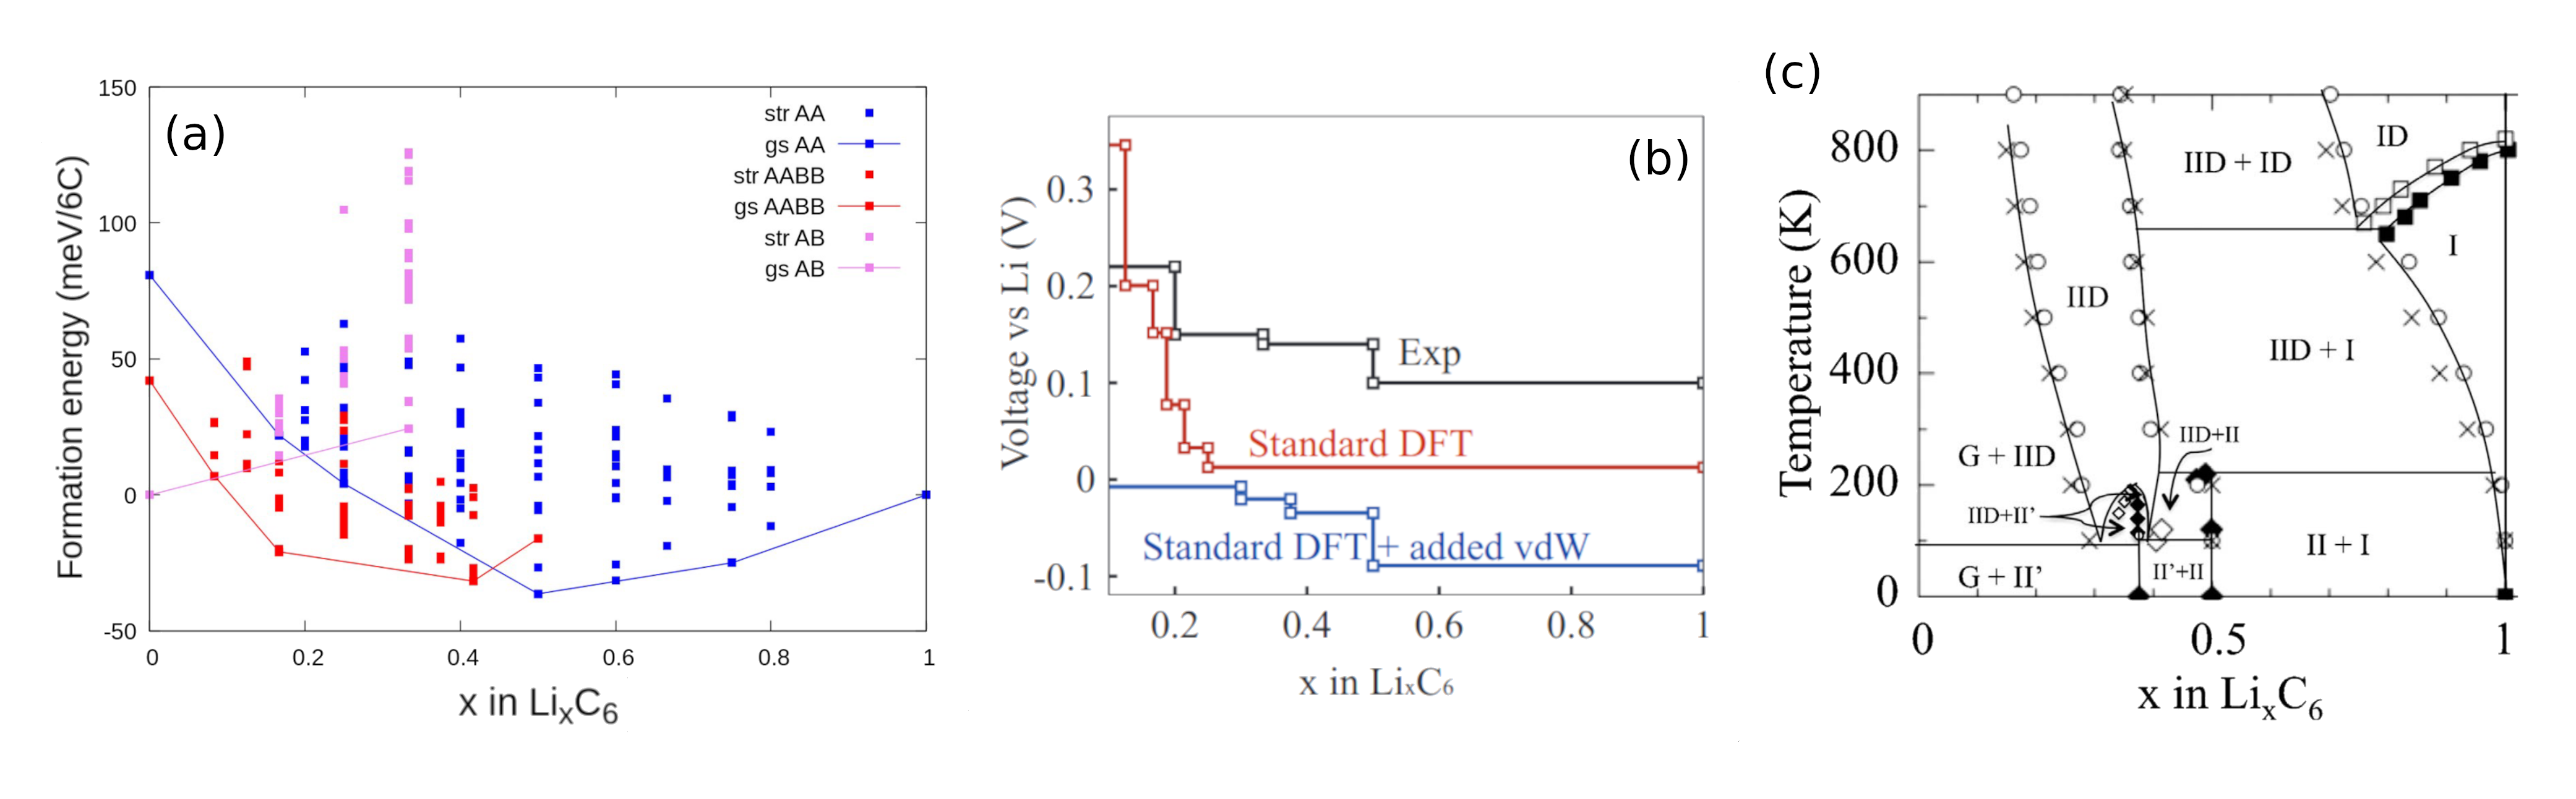
\includegraphics[scale=0.45]{figures/cluster_expansions_persson.png}
    \caption{(a) Formation energies of lithium in graphite performed with different carbon stackings. All calculated structures are denoted ``str'' while the ``gs'' represent the ground state structures in each of the three carbon stackings: AB, AABB, AA. (b) Phase diagram of lithium in graphite, determined by performing Monte Carlo calculations parameterised by effective cluster interactions from Density Functional Theory calculations. (c) zero kelvin equilibrium potential profiles dependent on different levels of van der Waals corrections. (a) Reproduced from Ref.~\citenum{Mercer2021} - Published by The Royal Society of Chemistry; (b-c) Reprinted with permission from Ref.~\citenum{persson2010}. Copyright 2010 American Chemical Society.}
    \label{fig:persson_graphitephases}
\end{figure}

The experimental OCV and the theoretical equilibrium potential are often, erroneously, considered to be equivalent. However, the OCV refers to the measured cell voltage without any external current and drifts with time. With sufficient time, it is often assumed the OCV will eventually relax to the equilibrium potential, but meta-stable states can occur that show no variation over experimental time scales of hours or even days.\cite{Liu2014,orisaka2013,Mercer2021} The true equilibrium potential, as defined in equation~\ref{eq:chemicalpotgibbs}, is a thermodynamic quantity and is not history-dependent \cite{VanderVen2020,Mercer2021}. Experimentally, a hysteresis of the measurable OCV between lithiation and delithiation is observed for Li/graphite half cells \cite{Ohzuku1993,Zheng1995,Dahn1991,Allart2018,Gallagher2012,Yazami_2006,GRIMSMANN201817,didier2020,Mercer2021} as shown in Figure~\ref{fig:expt_ocv}. Hysteresis is observed even after several hours of relaxation time and for $T > 298$ K, clearly demonstrating that the measured OCV is not a simple function of the thermodynamic ground state. Hysteresis therefore poses an interesting challenge to atomistic modellers.

It was recently shown that (de)-lithiation hysteresis in graphite is intimately connected with disorder in Stage II configurations and appears to be associated with a different carbon stacking pathway in each cycling direction \cite{Mercer2021}. Notably, energetic barriers to translate between ground state configurations, as determined through climbing image nudged elastic band (CI-NEB) calculations (Methods section~\ref{sec:methods_neb}), do not explain the hysteresis in graphite. Non-ground state configurations are involved in the delithiation direction. Understanding that behaviour requires the configurational entropy of Li/vacancy arrangements to be quantified, which is explained in more detail in the next section.  

\subsubsection{Entropy}
\label{sec:anodes_entropy}
The internal energy of intercalation electrodes arises largely from electrostatic interactions between the constituents. Those interactions can be well approximated by DFT. An atomistic description of the entropic behaviour of intercalation electrodes, $S(x)$, is also needed to correctly model thermal behaviour at $T>0$ K. The partial molar entropy, $dS(x)/dx$, is an experimentally accessible quantity, which can be probed by monitoring how the OCV, described in the previous section, varies with temperature (equation~\ref{eq:entropy_measurement}, c.f. refs. \citenum{Mercer2019,schlueter_quantifying_2018,Reynier2004,Yazami_2006,THOMAS2003844,OSSWALD2015270,Mercer2021} for further details). $S(x)$ is a sum of configurational, vibrational, and electronic components \cite{REYNIER2003850,Reynier2004}. For lithium in graphite, the electronic component can be neglected and the vibrational component can be well approximated by assigning a Debye temperature to all of the vibrational modes \cite{REYNIER2003850,Reynier2004}, or by computing phonon spectra from electronic structure methods \cite{hazrati_li_2014,vanderven2018} (c.f. section~\ref{sec:thermal_electronic_vibrational}). The quantity that shows the greatest difference with lithium concentration, $x$, is the configurational entropy of Li/vacancy arrangements, $S_{\rm{config}}$. Because of the staging phenomena described in section~\ref{sec:anodes_structure_stages}, $S_{\rm{config}}$ strongly deviates from ideal solid solution behaviour for Li in graphite.

The partial molar entropy $dS(x)/dx$ is difficult to interpret atomistically and so integration is required to get $S_{\rm{config}}$:

\begin{equation}
    \int_{x'=0}^{x'=x} \left(\frac{{\partial}S_{\rm{config}}(x')}{{\partial}x'}\right)dx' = S_{\rm{config}}(x) \approx S(x) - S_{\rm{vib}}(x),
    \label{eq:entropy_integration}
\end{equation}

where $S_{\rm{vib}}$ is the vibrational entropy approximated by Debye temperatures  \cite{REYNIER2003850,Reynier2004}. The integration constant is $S_{\rm{config}} = 0$ at $x=0$, because there can be no Li disorder in pure graphite. 

\begin{figure}
    \centering
    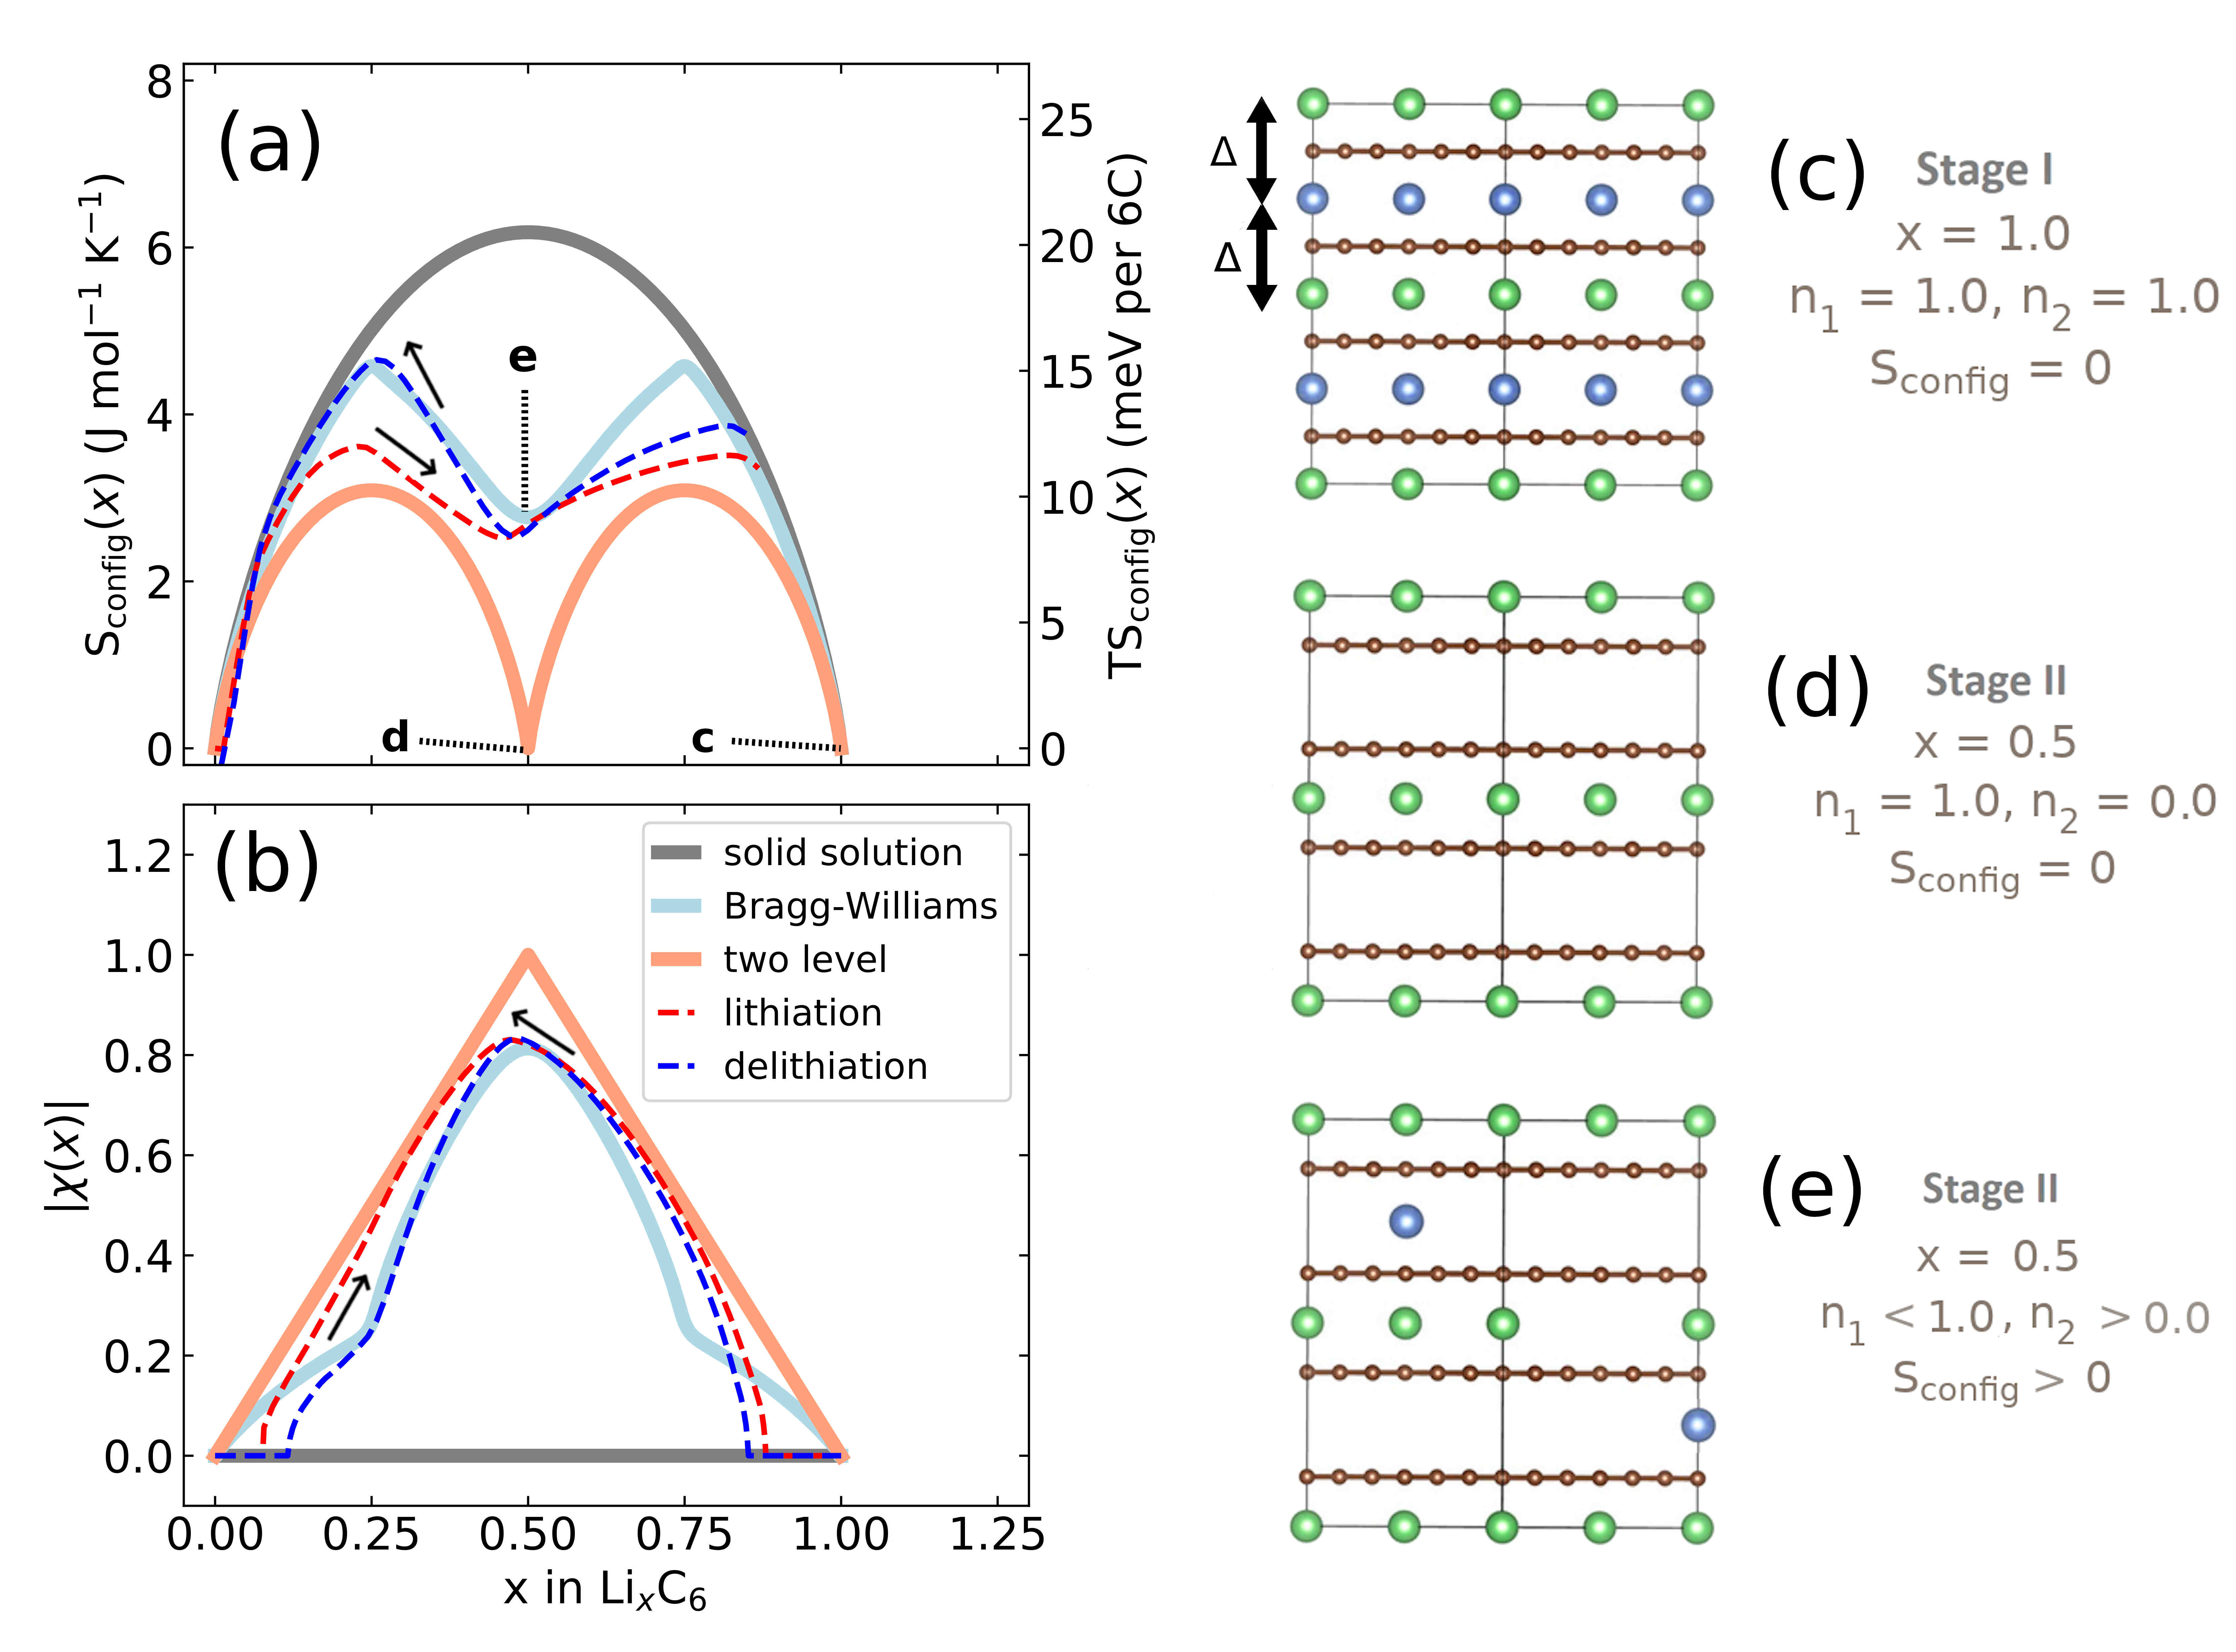
\includegraphics[scale=0.36]{figures/order_parameter_scheme_v2.jpg}
    \caption{(a) Configurational entropy obtained at $T$ = 320 K:~\emph{dark grey solid line}: ideal solid solution;~\emph{light blue solid line}: Bragg-Williams solution;~\emph{orange solid line}: sequential two level solid solution;~\emph{red dashed line}: experimental lithiation;~\emph{blue dashed line}: experimental delithiation. (b) Order parameter \textbar{}\(\chi\)\textbar{}, as described in the main text, labelled as in (a). In (a), select points (c-e) are indicated and schematic representations of the lattice occupations of Li in levels $n_{1}$ (green balls) and $n_{2}$ (blue balls) are shown on the right. Reproduced from Ref.~\citenum{Mercer2021} - Published by The Royal Society of Chemistry.}
    \label{fig:entropy_scheme}
\end{figure}

Dashed lines in Figure~\ref{fig:entropy_scheme}a denote post-processed experimental data obtained during lithiation and delithiation using equation~\ref{eq:entropy_integration} from ref. \citenum{Mercer2021}. Qualitatively, this shows more configurational Li disorder, i.e. larger entropy, is obtained during delithiation than lithiation. The lithium arrangements can be split into sublattice occupancies $n_{1}$ and $n_{2}$ arranged in alternate planes, as shown visually in Figure~\ref{fig:entropy_scheme}c-e. Each sublattice occupancy is linked to the degree of lithiation, $x$, via $x = (n_{1} + n_{2})/2$.

Solid lines in Figure~\ref{fig:entropy_scheme}a-b indicate three hypothetical cases. The orange solid line denotes solid solution (random) filling of Li into one of the sublattices for $x < 0.5$, followed by solid solution filling of the other sublattice, resulting in two maxima. Note that $S_{\rm{config}}$ is zero in Stage II at $x = 0.5$ (c.f. Figure~\ref{fig:entropy_scheme}d). The dark grey line shows the result for an ideal solid solution, if Li were to fill all available sites at random, i.e. $n_{1} = n_{2}$ for all $x$. The blue solid line is the solution to a Bragg-Williams model, \cite{Mercer2019,OTERO2017569} assuming only nearest neighbour repulsive pairwise lithium interactions between planes of $\Delta = 75$ meV and no in-plane interactions. That model allows a direct evaluation of the partition function (c.f. equation~\ref{eq:partition_fn}) by enumerating through all possible arrangements of Li atoms on the two sublattices for a given $x$ within the canonical ensemble. The out-of-plane Li-Li interactions are treated within a mean field (non-local) approximation to simplify the computation (details and formulae in refs.~\citenum{Leiva2017b,Mercer2019,OTERO2017569}).

The Bragg-Williams model produces a behaviour in $S_{\rm{config}}(x)$ between that expected for the solid solution and sequential two level filling. At $x = 1$, there is a net repulsion on each Li atom of 2$\Delta$, as represented in Figure~\ref{fig:entropy_scheme}c. At $x = 0.5$, one of the sublattices becomes preferentially filled, as represented schematically in Figure~\ref{fig:entropy_scheme}e. In contrast, a perfect Stage II structure as predicted by sequential two level filling (Figure~\ref{fig:entropy_scheme}d), would result in $S_{\rm{config}}(0.5) = 0$. 

These results can be understood within the framework of order parameters \cite{natarajan2017}. The relevant staging order parameter, $\chi(x) = n_{1} - n_{2}$, is shown in Figure~\ref{fig:entropy_scheme}b.  Formally, $\chi(x)$ takes values between $-1$ and $+1$, but only the absolute value is meaningful in this case. If $|\chi(x)| = 1$, then only one layer is filled with Li, representing maximal staging order. If $\chi(x) = 0$, both sublattices are occupied with equal probability, maximising disorder and hence no staging order is observed.

Greater interlayer Li disorder is observed during delithiation below $x = 0.5$. The Li ordering, as described by the order parameter, closely follows the Bragg-Williams model. This is expected if the host lattice remains in a metastable AA stacking. The lithiation behaviour shows a configurational entropy closer to solid solution filling of half the sites, which would be expected in AABB stacking, since only half the interlayers (i.e. those locally adopting AA or BB stacking) provide favourable Li insertion sites. As shown in Figure~\ref{fig:persson_graphitephases}a, this is the ground state stacking configuration for $x < 0.5$.

The wider implication of these results is that the transformations between the stackings in graphite, and possible stacking dynamics in other layered intercalation hosts, deserve more attention. These phase transformations not only create a challenge from a cell diagnosis point-of-view, they could also be partially responsible for mechanical degradation, fracture, unstable interfaces and loss of active material. Phase transformations should be described in a rigorous way in continuum models. It is not sufficient to approximate the guest ions as an ideal solid solution as, for instance, done in the popular Doyle-Fuller-Newman (DFN)-type models. 

\hlcyan{It is worth noting that the host lattice ordering of graphite obtained in electrochemical conditions is difficult to access from experimental analysis. In-operando x-ray and neutron diffraction experiments allow the interlayer carbon separation to be obtained.}\cite{Billaud1996,BILLAUD2002299,Woo1983,Dahn1991,Ohzuku1993,didier2020} \hlcyan{However, it is extremely difficult to obtain the stacking displacements within each carbon layer, as the superstructure peaks associated with these displacements}\cite{Konar2015} \hlcyan{are weak and obscured by peaks from the current collector.}\cite{didier2020,Senyshyn2013,Taminato2016} \hlcyan{A reason as to why there is still some dispute in the literature regarding the Li-graphite stages of order greater than 2, as highlighted earlier in} \ref{sec:anodes_structure_stages}, \hlcyan{is that these in-plane displacements cannot be completely elucidated.} \hlcyan{These displacements influence the lithium ordering in each atomic layer, which is even harder to determine than the carbon ordering and is currently not feasible even in neutron diffraction experiments. It is also not possible to determine this information through local probes such as nuclear magnetic resonance (NMR) and Raman scattering.}\cite{Sole2014,lopez2018} \hlcyan{It is only through the combination of atomistic and statistical mechanical models, together with entropy profiling measurements, that the proportion of lithium in the different layers in Stage II configurations could be quantified.}\cite{Mercer2021} \hlcyan{With regard to systems other than lithium-graphite, atomistic techniques could enable lithium guest orderings to be quantified by means of order parameters, which,  for the reasons explained above, is information inaccessible through experiment alone. Synergies between models of host and guest ion orderings with appropriate experimental characterisation will enable a new generation of modelling tools that can predict these phenomena with greater accuracy.} \cite{franco2019,VanderVen2020}

As shown in the next section, orderings in Li-GICs have implications for the dynamics of Li intercalation as well.

\subsubsection{Ion diffusion in Li-GIC} 
\label{sec:anodes_ion_diffusion}

Having outlined the use of atomistic techniques to evaluate observable thermodynamic properties of anodes and, in particular, graphite, this section focuses on the computation of bulk dynamic properties by DFT and kMC approaches.

Li diffusivity is similar for stage I and stage II Li-GICs, \cite{persson2010} with the probable Li migration pathways for LiC$_{6n}$ illustrated in Figure~\ref{fig:Rl}.  \cite{thinius2014theoretical} These pathways were determined from DFT calculations within a CI-NEB approach. Here, Li diffusion across the graphite layers through a carbon hexagon hollow (H) are denoted as the through-plane pathway. The in-plane or two-dimensional Li migration along the crystallographic ab plane occurs either by a bridge (B) migration pathway, where Li passes through a rectangle of carbon atoms of subsequent layers, or a top (T) migration pathway, where Li passes in between two congruent carbon atoms. 

\begin{figure}
    \centering           
    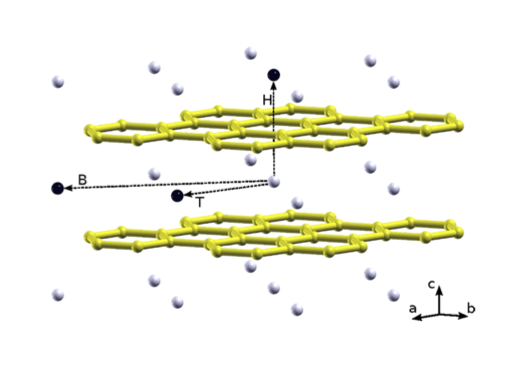
\includegraphics[scale=0.8]{figures/Islam-Fig-LiC6.png}
    \caption{Li migration pathway in LiC$_{6}$. In the through-plane pathway, lithium migrates through a carbon hexagon hollow (H) along the crystallographic c direction. The in-plane pathways are denoted as bridge (B) and top (T). Reprinted (adapted) with permission from Ref.~\citenum{thinius2014theoretical}. Copyright 2014 American Chemical Society.}
    \label{fig:Rl}
\end{figure}

Diffusion proceeds in the aforementioned through-plane pathways and in-plane pathways via the Frenkel and vacancy mechanisms, respectively. \citeauthor{thinius2014theoretical} showed that Li diffusion along the crystallographic $c$ direction is kinetically prohibited, due to a large activation energy barrier.\cite{thinius2014theoretical} The calculated activation energy for this migration pathway is extremely high (8.00 -- 8.23 eV), therefore, the Boltzmann probability for diffusion through pristine graphene planes is negligible at $T = 300$ K. It is therefore likely that diffusion in the $c$ direction occurs via grain boundaries. \cite{persson2010lithium} In contrast, the activation energy for Li diffusion in the crystallographic ab plane is much lower (0.42 -- 0.52 eV), showing that in Li-GICs, Li diffuses mostly within the intercalation layers.\cite{thinius2014theoretical} In the literature, DFT-based theoretical investigations provide the same qualitative trends for ion diffusion mechanisms in Li-GICs and the calculated activation barriers vary slightly, but are within the same order of magnitude.\cite{Imai-JAC-2007,persson2010lithium,toyoura2010effects,Wang} 

In order to gain insights into the Li diffusion process in graphite, far from equilibrium and under fast charging conditions, \citeauthor{Hakim} simulated a range of compositions between stage I and IV, i.e. dilute Stage I.\cite{Hakim} Their study determined reduced activation barriers in the in-plane migration pathways (0.2 -- 0.32 eV), which is attributed to the presence of a higher number of electrons compared to Li$^{+}$ ions, occurring at the very beginning of the lithiation cycle during fast charging conditions. This extra charge increases the interlayer spacing in the diffusion layer and adjacent channels, increasing the Li diffusivity.\cite{Hakim} \citeauthor{JI201866} investigated the anisotropic strain effects on lithium diffusion in graphite anodes using DFT and kMC simulations. \cite{JI201866} According to their study, the activation energy for Li diffusion in unstrained Li$_{x}$C$_{6n}$ is 0.48 eV. The tensile strain along the direction perpendicular to the graphite planes facilitates in-plane Li diffusion by reducing the energy barrier and vice versa.\cite{JI201866}

\citeauthor{gavilan-arriazu_kinetic_2020} have recently simulated the dynamic properties of lithium intercalation in graphite using kMC \cite{gavilan-arriazu_kinetic_2020, gavilan-arriazu_effect_2020,GAVILANARRIAZU2018133}. These models considered exchange of Li with the solution on one side of a slab (Figure~\ref{fig:graphite_kmcscheme}), with only interplanar Li transport allowed, based on the diffusion barrier arguments presented above. Energetic barriers for Li exchange into/out of the graphite were calculated assuming Butler-Volmer kinetics, based on experimental exchange current density data. Interplanar diffusion barriers were computed using random walk theory, based on experimental data in the dilute limit. Respective barriers of 0.655 eV and 0.370 eV for exchange and interplanar diffusion were obtained. This approach enabled the simulation of several different dynamic properties dependent on lithium concentration, $x$, \cite{gavilan-arriazu_kinetic_2020,gavilan-arriazu_kinetic_2020} sweep direction \cite{gavilan-arriazu_kinetic_2020}, and temperature \cite{gavilan-arriazu_effect_2020}, with a few of these highlighted in Figure~\ref{fig:graphite_kmcobservables}. Additionally, the importance of metastable Daumas-H\'{e}rold orderings in Stage II configurations \cite{GAVILANARRIAZU2018133} and clogging of lithium at the interface \cite{gavilan-arriazu_kinetic_2020} leading to slow Li insertion kinetics were identified as important challenges limiting the kinetics of the lithium (de)insertion processes.

\begin{figure}
    \centering
    \includegraphics[scale=2]{figures/kmc_scheme.png}
    \caption{Representation of insertion and diffusion of lithium in graphite in a kinetic Monte Carlo model. Reproduced from Ref.~\citenum{gavilan-arriazu_effect_2020} - Published by the Journal of The Electrochemical Society.}
    \label{fig:graphite_kmcscheme}
\end{figure}

\begin{figure}
    \centering
    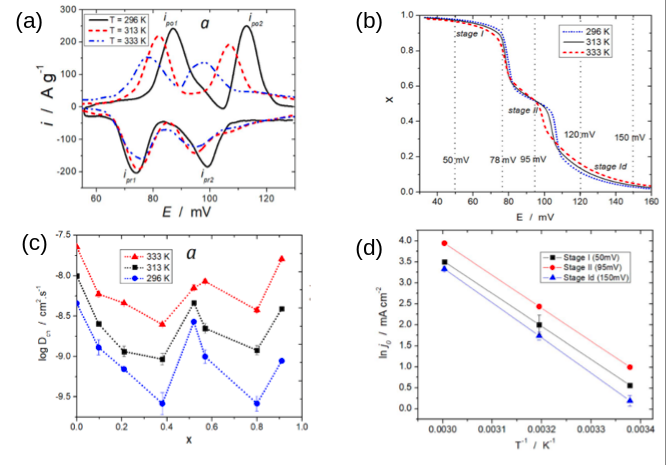
\includegraphics[scale=2]{figures/kmc_observables.png}
    \caption{Effect of temperature on the dynamic behaviour of lithium insertion in graphite. (a) voltammograms (b) voltage profiles (isotherms) (c) diffusion coefficients, (d) exchange current density. insertion and diffusion of lithium in graphite in kMC model. Reproduced from Ref.~\citenum{gavilan-arriazu_effect_2020} - Published by the Journal of The Electrochemical Society.}
    \label{fig:graphite_kmcobservables}
\end{figure}

Having described modelling of the thermodynamics and bulk Li diffusion in graphite, the following section will focus on another important aspect for a multiscale model: the structure and dynamics of the graphite edges.

\subsection{Graphite Surfaces and Interfaces}
\label{sec:anodes_surfaces_interfaces}

\subsubsection{Possible graphite surfaces and their stability}
As discussed above, investigating the bulk properties of lithium is key to understanding Li intercalation kinetics and (dis)charging rates in graphite. However, Li exchange occurs between the graphite surfaces and the electrolyte, hence a multiscale model needs to include these phenomena. Addressing the surface properties of graphite would improve the understanding of (dis)charging behaviours at graphite anodes and possibly suggest how to enhance the (dis)charging rates.

As shown in Figure~\ref{fig:graphite_surfs} and section~\ref{sec:anode_bulk}, graphite consists of multiple stacked graphene layers. One of the exposed surfaces is the basal plane or the (001) surface, which has been widely investigated in both the theoretical and experimental studies.\cite{thinius2014theoretical,persson2010,toyoura2010effects,yao2012diffusion,nuli2006intercalation} In contrast, the non-basal planes attract less attention, due to their complicated edge morphology. Recently, experimental studies characterised the SEI formation and growth along the graphite edges as opposed to the basal plane, \cite{liu2019situ,zhang2020operando} indicating the importance of the graphite non-basal plane for facilitating Li intercalation.

\begin{figure}
    \centering
    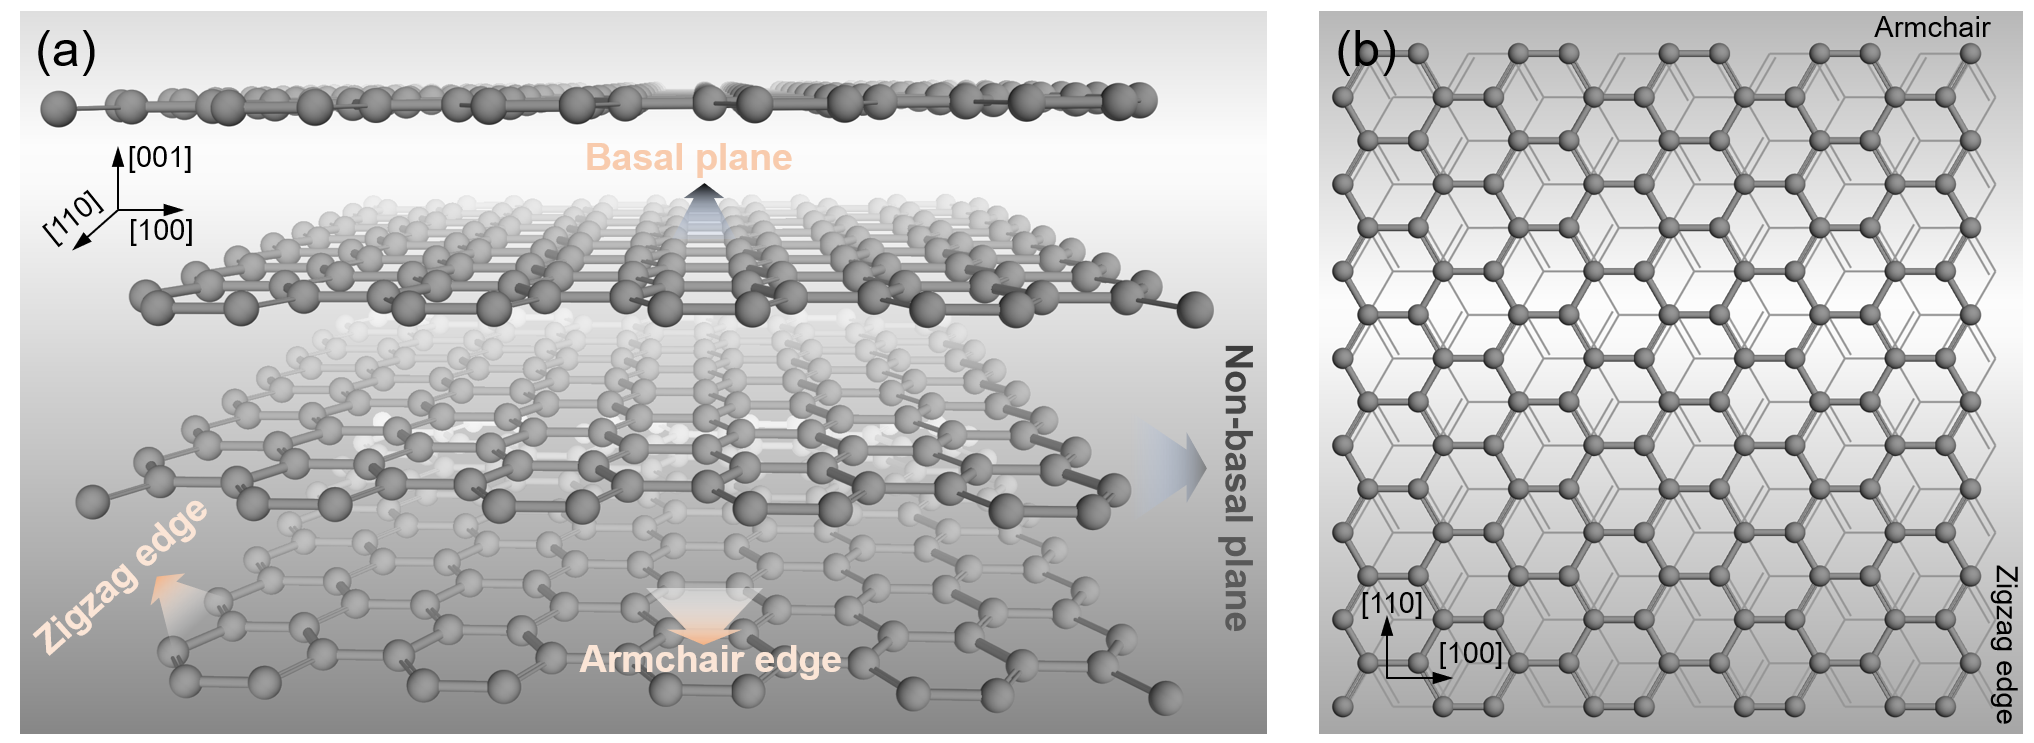
\includegraphics[scale=0.4]{figures/Graphite_surfs.png}
    \caption{(a) structures of the basal plane and the non-basal plane of graphite. The latter plane consists of different edges of graphites, such as armchair edge and zigzag edge. (b) topological geometries of graphite edges.}
    \label{fig:graphite_surfs}
\end{figure}

\citeauthor{Rana-Graphite-Surf} investigated the stability of various low index graphite surface planes including the (001), (110), and (100) planes. The calculations were performed using dispersion corrected DFT approaches.\cite{Grimme-2,Grimme-4} The surface energies of these planes were found to go in the order (001) $<$ (110) $<$ (100), \cite{Rana-Graphite-Surf} indicating that the (001) surface (the basal plane) is the most energetically favourable. However, this plane does not favour Li intercalation, due to the high diffusion barrier required for Li to go through the carbon hexagon \cite{thinius2014theoretical,persson2010}, as highlighted in the previous section on ion diffusion in Li-GICs (sec~\ref{sec:anodes_ion_diffusion}. Li intercalation of graphite particles must therefore proceed either via defects in the (001) plane or via the non-basal planes.

The (100) surface consists of nanoribbons with a zigzag edge, whereas the (110) surface adopts an armchair conformation. The relatively unstable surface planes, such as the (100) plane, can be stabilised by various procedures, including chemisorption of oxygen atoms.\cite{Rosanna} It was found that the oxygen functional groups not only stabilise the graphite edges, but are also critical for the formation of the SEI layer near the edge, thereby preventing graphite exfoliation.\cite{bernardo2015influence} Investigating those non-basal planes and their effects on Li intercalation are therefore important and are addressed in the following section.

\subsubsection{Surface Effect on Intercalation Energy} 
Understanding the nature of Li intercalation in graphite is important for optimisation of the anode material. As described above, Li intercalation in the bulk of graphite has been widely investigated.\cite{persson2010,toyoura2008first,toyoura2010effects,yao2012diffusion,thinius2014theoretical} Experimental Li diffusivities in graphite have been reported, ranging from $10^{-6}$ -- $10^{-14}$ cm$^2$ s$^{-1}$.\cite{toyoura2010effects, takami1995structural, yang2004evaluation,yu1999determination} However, DFT calculations\cite{persson2010} based on bulk graphite indicate that Li diffusion coefficients based on the AABB and AA stacked graphite are around 10$^{-7}$ cm$^2$ s$^{-1}$ and decrease slightly with increasing Li concentration.\cite{persson2010} The variability between reported experimental diffusion coefficients arises from a combination of the staging dynamics and the anisotropy of Li diffusion (through versus into the basal plane). There is also a difference between the surface morphologies of different types of graphite, i.e. the proportion of zigzag and armchair edges and their surface chemical terminations, implying possible differences between the electronic behaviour and charge transfer kinetics dependent on edge morphology and termination. Therefore, investigation beyond the bulk properties of graphite is necessary to optimise the overall rate performance of graphite electrodes. As described in section~\ref{sec:anodes_surfaces_interfaces}, the basal plane is relatively inert towards Li intercalation.\cite{persson2010lithium} The non-basal plane, consisting of different edge morphology, attracts more attention due to observations of Li intercalation and SEI growth.\cite{liu2019situ,zhang2020operando} \citeauthor{uthaisar2010edge} studied the Li adsorption and diffusion on the edged graphene system using DFT.\cite{uthaisar2010edge} The graphene edges were found to affect not only Li adsorption but also the diffusion coefficient. Narrower graphite nanoribbons showed faster delithiation behaviour than the larger sized graphene, due to the topological effect of graphene edges. This highlights that an in-depth knowledge of interface effects is needed to understand Li intercalation rate and enable rational optimisation of the battery performance.

\begin{figure}
    \centering
    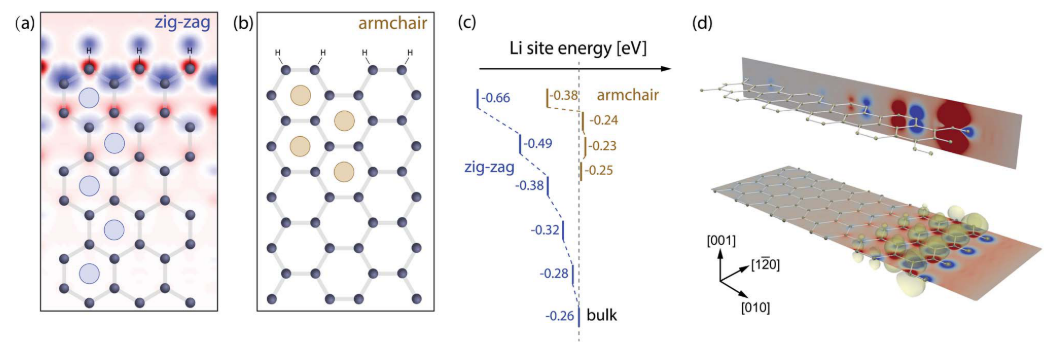
\includegraphics[scale=0.6]{figures/Intercalation energies.PNG}
    \caption{Structures of the zigzag-edged graphite (a) and the armchair-edged graphite (b). (c) shows the energy profile of Li adsorption in edged graphite. (d) is the spin densities of zigzag-edged graphite. The iso-surface value is 0.0002 e \AA$^{-3}$. Reproduced from Ref.~\citenum{peng2020lithium} with permission from The Royal Society of Chemistry.}
    \label{fig:arm_zig}
\end{figure}

From an atomistic perspective, the surface and edge morphology of anode materials were found to have a strong impact on Li binding energies.\cite{uthaisar2010edge,leggesse2016lithium} Through investigating Si nano-structures, \citeauthor{chan2010controlling} found that Li has higher binding energies at the bulk site compared to the edge, requiring a higher energy cost of Li migration from the bulk towards the edge.\cite{chan2010controlling} In graphite anode materials, however, \citeauthor{leggesse2016lithium} reported that the edged graphite systems showed remarkably enhanced Li binding energies and high Li mobility along graphite edges.\cite{leggesse2016lithium} \citeauthor{peng2020lithium} recently quantified the edge effects on Li intercalation in graphite.\cite{peng2020lithium}. In their work, different edged graphites at dilute Li concentration were comprehensively investigated using DFT calculations. Interestingly, they found the unique topological electronic structures near the edges, particularly near the zigzag edge, induced distinct intercalation energies of Li in graphite. Figure~\ref{fig:arm_zig}c shows the Li adsorption energies at the armchair-edged and the zigzag-edged graphite, respectively. The adsorption energy, $E_{\rm{ads}}$, is expressed as:

\begin{equation}
    E_{\rm{ads}} = E_{\rm{Li|Graphite}}-E_{\rm{Graphite}}-E_{\rm{Li}},
    \label{eq:adsorption_energy}
\end{equation}

where $E_{\rm{Li|Graphite}}$, $E_{\rm{Graphite}}$, and $E_{\rm{Li}}$ are the energies of Li adsorption in graphite, the pristine graphite, and one Li in body-centred cubic (bcc) Li metal, respectively. At the armchair edge, from the energy profile (c.f. Figure~\ref{fig:arm_zig}), the adsorption energy of Li is the lowest at the edge site (-0.38 eV). With Li penetrating into the bulk, the adsorption energy decreases rapidly to -0.24 eV at the sub-surface site and becomes -0.26 eV at the bulk site. The topological geometry of the armchair edge promotes Li adsorption relative to the graphite bulk.

At the zigzag edge, the edge effect becomes even stronger, due to the existence of the surface state which consists of ${\rm{C}}-p_{\rm{z}}$ orbitals emerging from the zigzag edge.\cite{fujita1996peculiar,lee2005magnetic} Figure \ref{fig:arm_zig}c shows that Li achieves a much lower adsorption energy of -0.66 eV at the zigzag edge site, indicating the strong binding of Li at the edge. The edge effect in the zigzag system is much stronger than that at the armchair edge and additionally penetrates into the bulk, indicated by the gradual decrease in magnitude of the Li adsorption energy from the edge to the bulk. 

The zigzag edge displays completely different spin densities contributed by the $p_z$ orbitals perpendicular to the graphene planes, as shown in Figure~\ref{fig:arm_zig}a-b. \cite{leggesse2016lithium,fujita1996peculiar,lee2005magnetic,peng2020lithium} These spin densities consist of the unpaired electrons accumulating on the edged carbons. The amplitude of this topological surface state gradually diminishes over a few bond distances beneath the surface. It is this surface state that interacts with Li at the zigzag edge and favours its adsorption. In summary, the graphite edges show stronger interactions with Li than those in the bulk. The effect is especially pronounced at the zigzag edge, strongly stabilising Li binding due to the topological surface states.
    
\subsubsection{The Surface Effect on Li Diffusion}
As Li obtains higher binding energies at the graphite edge, due to the specific topological structure of graphite edges,\cite{leggesse2016lithium,peng2020lithium} it's worth examining the impact of those edges on Li diffusion. In bulk graphite, the diffusion barrier of Li jumping from one site to another is around 0.4 eV at the dilute limit.\cite{thinius2014theoretical} Li, however, exhibits completely different diffusion kinetics at graphite edges in contrast to those in the bulk.\cite{leggesse2016lithium,peng2020lithium} 

\citeauthor{peng2020lithium} show the energy profile of Li diffusion from the graphite edge towards the bulk at dilute Li concentration, Figure~\ref{fig:Li_diffusion_edge}. In the armchair-edged graphite, Li has to overcome an energy barrier of 0.43 eV to move from site 1 to site 2 and a 0.42 eV barrier to further move from site 2 to site 3. The direct jump from site 1 to site 3 has to overcome an energy barrier of 0.58 eV and is therefore less favourable. In contrast, for bulk diffusion, Li needs to overcome a $\sim$0.43 eV barrier to move to either adjacent site. The higher diffusion barrier at the armchair edge is caused by the compensation of Li adsorption energy at the edge site. At the zigzag edge, Li obtains two different diffusion pathways. Li diffusion from the edge (site 1) to the subsurface (site 3), where the diffusion barrier is 0.48 eV. In contrast, there is only a 0.21 eV activation barrier for Li diffusion along the edge sites (site 1 to site 2), which is much lower. This indicates that Li is extremely mobile at the zigzag edge, which can be verified by the stronger flux connecting the edge sites compared to diffusion towards the bulk (c.f. Figure~\ref{fig:Li_diffusion_edge}). Due to the surface effect identified at the zigzag edge, Li favours diffusion along the edge direction within the first sub-surface sites, as the diffusion barrier (0.41 eV) is still lower than the barrier to moving Li into the bulk (0.49 eV). Markov chain analysis was conducted in \citeauthor{peng2020lithium}'s study to examine Li diffusion from the armchair edge and the zigzag edge to a bulk site 20 \AA \ below the edge surface (see Figure \ref{fig:Li_diffusion_edge}c). They demonstrated that Li diffusion from the armchair edge to the bulk site is around one order of magnitude faster than its diffusion from the zigzag edge to the bulk, due to the strong binding of Li at the zigzag edge that generates a deep potential well for Li.\cite{peng2020lithium}

On the basis of these studies, it was shown that the graphite edges have strong effects not only on the Li intercalation energies but also on its diffusion kinetics close to the edge.\cite{leggesse2016lithium,peng2020lithium} The effect is pronounced at the zigzag edge.\cite{bernardo2015influence,velicky2019electrochemistry,gerischer1985interpretation} Thus much more sluggish (de)intercalation kinetics are expected at that edge, compared to the armchair edge. Strategies including promoting growth of armchair edge over zigzag edge during synthesis of graphite nanomaterials,\cite{bernardo2015influence} and tuning the edge properties by chemical doping to improve Li diffusion rate towards the bulk could be useful to enhance Li (dis)charging rate for graphite anodes.\cite{weydanz1994behavior,way1994effect,endo2001scanning} 

\hlcyan{Designing edge-controlled graphite for validating the electronic and electrochemical properties predicted by DFT is still state-of-the-art. Commercial graphite powders contain a distribution of sizes, the proportion of edge types on each particle is dependent on particle size, and it is currently not possible to form graphite with only one type of edge. This makes systematic experimental characterisation to determine the influence of edges difficult.}\cite{ishii2017}  \hlcyan{To try to understand these effects} \citeauthor{bernardo2015influence} \hlcyan{studied the effect of hydrogen and oxygen gas etching on graphite materials with a higher incidence of zigzag or armchair edge orientations.}\cite{bernardo2015influence} \hlcyan{The proportion of each edge was quantified by high resolution transmission electron microscopy (HR-TEM), with the authors finding that a higher proportion of zigzag edges leads to a less stable SEI.} \citeauthor{velicky2019electrochemistry} \hlcyan{studied the local electron transfer rate, double layer capacitance, and local density of states of the edge versus the basal plane of graphite in a microdroplet electrochemical cell.}\cite{velicky2019electrochemistry} \hlcyan{This study was feasible owing to the vastly different electronic structure and electron transfer rate constant of the basal plane versus the graphite edges. It has yet to be determined if it is currently feasible to distinguish these properties for the zigzag and armchair edge, in a real electrochemical environment, through such an approach. Even so, the finding that the surface state from the zigzag edge could be a major bottleneck to the Li intercalation rate is a triumph for atomistic modelling that could direct future materials design strategies and experimental characterisation for anodes.}\cite{peng2020lithium,peng2021} \hlcyan{Moreover, the interplay between edge orientation and nitrogen/boron doping warrants further systematic exploration from both experiment and theory}.

These studies can also offer some universal insights for investigating the interface effects of other materials such as the cathode. Prior to Li intercalation into graphite, the Li desolvation process is also an important step affecting the overall (dis)charging rate. However, due to the complicated solid-liquid interface, addressing the graphite interaction with the electrolyte is an extremely challenging aspect for both modelling and experiment, as discussed in the following sections. We discuss the effect of that interface on Li plating and aspects related to the SEI in the following sections.

\begin{figure}
    \centering
    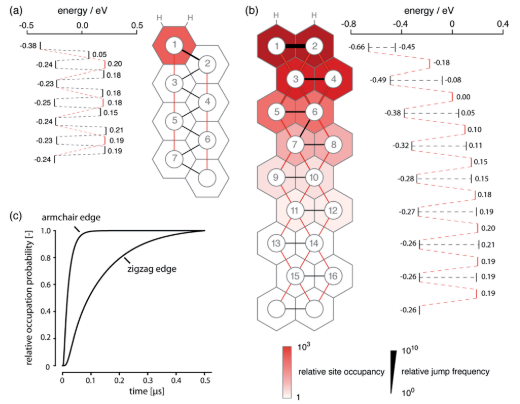
\includegraphics[scale=0.5]{figures/Graphite_edge_effects.PNG}
    \caption{Li diffusion at (a) the armchair-edged and (b) the zigzag-edged graphite. The hexagons indicate lattice sites and the colours show occupancy probability relative to that in the bulk. The width of the lines connecting sites implies the jump frequencies. (c) shows the occupation probability for Li to occupy a site approximately 20 \AA \ below the graphite edge, relative to the steady-state value after being introduced at time zero at the edge. Reproduced from Ref.~\citenum{peng2020lithium} with permission from The Royal Society of Chemistry.}
    \label{fig:Li_diffusion_edge}
\end{figure}

\subsubsection{Li deposition on graphite anodes}
\label{sec:li_deposition}

Apart from intercalation of Li ions into the graphite anode, Li ions can also deposit on surface of graphite in the form of metallic Li dendrites, which can grow during battery operation and cause internal short-circuits. Several situations for the deposition of Li metal on the graphite anode have been identified, as shown schematically in Figure~\ref{fig:li_plating}.\cite{Gao2021} A ``normal'' intercalation mechanism is shown in Figure~\ref{fig:li_plating}a. When the voltage of the graphite electrode drops below 0~V with respect to Li/Li$^+$, deposition of Li$^+$ ions on the graphite surface, as metallic Li, becomes thermodynamically possible, as shown in Figure~\ref{fig:li_plating}b. The thermodynamic criterion can be satisfied when the overpotential, $\eta_{int}$, is larger than the equilibrium voltage of the stage II to stage I phase transition ($\sim$85~mV). Deposition becomes kinetically feasible when the overpotential for the intercalation reaction ($\eta_{int}$) becomes larger than the intercalation voltage ($\sim$85~mV), so that the graphite voltage drops below 0~V with respect to Li/Li$^+$. The overpotential originates from mass transfer limitations in the electrolyte region near the graphite edge, as shown schematically in Figure~\ref{fig:li_plating}c. Li plating can be triggered upon local salt depletion in the electrolyte, $c_l\rightarrow 0$, if liquid diffusion is slow compared to intercalation. Solid-state diffusion between the graphite edge and the bulk, as shown schematically in Figure~\ref{fig:li_plating}d, also contributes to this overpotential.  Li plating can occur when intercalated Li$^+$ ions saturate the graphite edge ($c\rightarrow1$) and block further insertion, if diffusion from surface to the bulk is slow compared to Li insertion at the edge. A combination of both effects can result in Li deposition on the graphite surface.

A recent DFT study by \citeauthor{peng2021} has shown that in a vacuum environment: (1) Li deposition is more favourable near the graphite edges rather on the basal plane, (2) the energy barrier for Li deposition at the zigzag edge (only) increases with the degree of lithiation of the graphite, (3) chemical doping of nitrogen can increase the energy barrier and can possibly suppress the Li deposition on graphite anode on the zigzag edge.\cite{peng2021} More advanced models for DFT simulations in the presence of an electrolyte under applied potential (cf. (sec.~\ref{sec:dft+cont} and Ref.~\citenum{Bhandari2021})), have the potential to shed more light on the Li deposition phenomenon in experimental conditions.

\begin{figure}
    \centering
    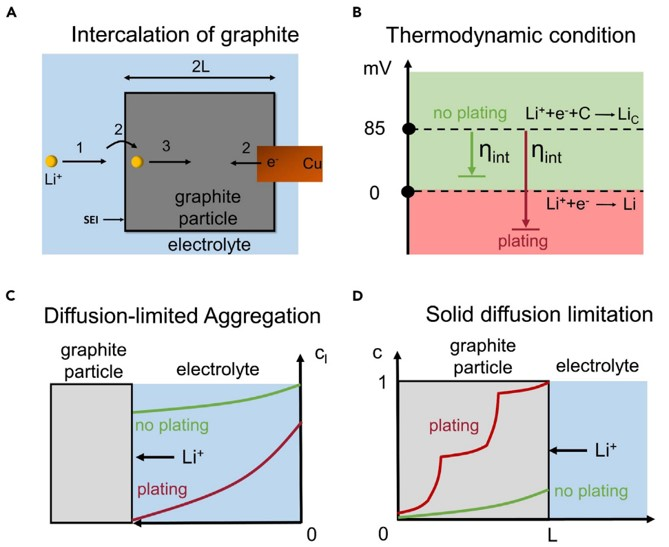
\includegraphics[scale=0.75]{figures/li_plating.jpg}
    \caption{(a) 2D schematic of intercalation of a graphite particle. Three sequential steps take place during charging at the graphite anode: (1) Li$^+$ transport in electrolyte toward the reaction site; (2) Li$^+$ intercalation into a graphite particle (including de-solvation and migration through the SEI); and (3) Li$^+$ solid diffusion within the graphite particle. (b) Thermodynamic criterion for Li plating (cell voltage, $U < 0$ V versus Li/Li$^+$). The green and red arrows illustrate the required overpotentials to drive the insertion reaction at small current/fast insertion kinetics and large current/slow insertion kinetics. (c) 1D schematic of diffusion-limited aggregation resulting from electrolyte transport limitations. The green and red curves illustrate the Li$^+$ salt concentration profile in the electrolyte. (d) 1D schematic of solid diffusion-limitation mechanism. The green and red curves illustrate the Li$^+$ concentration profile in the graphite particle. Reprinted from Ref.~\citenum{Gao2021}, with permission from Elsevier.}
    \label{fig:li_plating}
\end{figure}

\subsubsection{Solid-Electrolyte Interphase}
\label{sec:SEI}
The SEI is an important component of the rechargeable Li-ion battery and is formed from deposition of the decomposition products of the electrolyte and solvent on the anode surface. The SEI allows transport of Li$^+$ ions but blocks the transfer of electrons, thereby stopping further electrolyte decomposition reactions.\cite{Winter2009, VERMA20106332} Here we discuss aspects of the SEI related to our discussion of Li-ion diffusion energy barrier in bulk and graphite surfaces. A recent comprehensive review on the atomistic modelling of the SEI describes several other aspects of the SEI in detail:\cite{Wang2018} 
\begin{itemize}
    \item Electrolyte and solvent reduction mechanisms, including: prediction of the reduction voltage for each solvent and electrolyte species, the effect of the electrolyte solvation structure, the effect of anode surface termination, and the dynamic buildup of the nanometer thick SEI layer.
    \item Modification of the SEI by electrolyte additives and prediction of new electrolyte additives.
    \item Correlation of the SEI properties with battery performance, including: the electron insulating properties of the inorganic components in the SEI, the ionic conductivity of the SEI components, Li-ion desolvation at the SEI/electrolyte interface, chemical stability of the SEI components, and mechanisms of SEI growth and battery aging.
    \item The use of coatings to artificially design the SEI.
\end{itemize}

One way to describe the SEI is via the implicit continuum models described in sec.~\ref{sec:dft+cont}. Applying their DFT + implicit electrolyte model on an armchair edge of 1634-atom graphite slab in contact with a 0.5 M LiPF$_6$ in EC solution, \citeauthor{Dziedzic2020} calculated that a Li atom is 2.34 eV more stable at the graphite edge than in the electrolyte solution.\cite{Dziedzic2020} Similarly, \citeauthor{haruyama2018} found favourable energetics for Li intercalation from the electrolyte solution into the graphite edge.\cite{haruyama2018} They also studied the variation in energy as a function of Li distance from the graphite edge, as shown in figure \ref{fig:gel}. In \citeauthor{haruyama2018}'s model, Li intercalation is accompanied by an electron gain from the external circuit. This was implemented using a grand canonical version of electronic DFT, where the number of electrons in the electrode can change subject to fixed electrode potential. Correspondingly, the appropriate thermodynamic quantity to represent this ensemble is the grand potential, $\Omega=A-\mu_e N_e$, which is plotted on the y axis for several different constant chemical potentials of electrons, $\mu_e$. Two illustrative cases include: (a) the potential of zero charge (PZC), which is the electrochemical potential of a charge-neutral Li-graphite system, and (b) the equilibrium potential (c.f.  sections~\ref{sec:properties_equilibriumvoltage} and ~\ref{sec:anodes_ocv}), where the net change in the grand potential for the intercalation reaction becomes zero. \citeauthor{haruyama2018}'s simulations estimate an energy barrier of around 0.6 eV for Li intercalation into the graphite edge, which is close to the experimental measurements from impedance spectroscopy.\cite{Yamada2009}

\begin{figure}
    \centering
    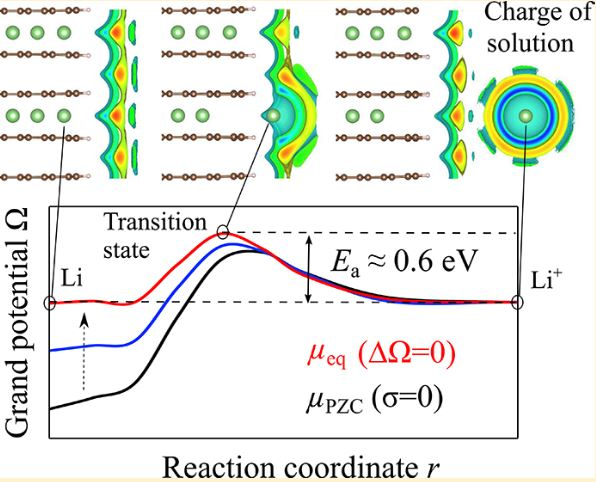
\includegraphics[scale=0.6]{figures/graphite-interface.JPG}
    \caption{Profiles of grand potential $\Omega$ as a function of the Li-position during Li-intercalation process at the interface between graphite edge and an implicit electrolyte solution. The simulation is performed at conditions of constant chemical potential of electrons $\mu_e$ (constant electrode potentials similar to experiments). Reprinted with permission from Ref.~\citenum{haruyama2018}. Copyright 2018 American Chemical Society.}
    \label{fig:gel}
\end{figure}

Another way to describe the SEI is via explicit consideration of SEI components. \citeauthor{Shi2012} performed a direct calculation of Li-ion transport in the Li$_2$CO$_3$ component of the SEI,\cite{Shi2012} via DFT-based CI-NEB calculations (section~\ref{sec:methods_neb}). Two mechanisms for Li$^+$ diffusion were considered, namely, the knock-off and direct hopping mechanisms, which were found to have energy barriers of 0.31 eV and 0.54 eV respectively, as shown in Figure~\ref{fig:sei}. The Li self-diffusion coefficient was calculated to be $1.1\times10^{-7}$ cm$^2$ s$^{-1}$ and $8.4\times10^{-12}$ cm$^2$ s$^{-1}$ respectively. Estimating the formation energy of corresponding defects in the lattice of Li$_2$CO$_3$ as a function of voltage, the total activation energy barrier for Li-ion diffusion was predicted to be in the 0.67--1.07 eV range for the knock-off mechanism and in the 0.92--1.32 eV range for the direct-hopping mechanism.

\begin{figure}
    \centering
    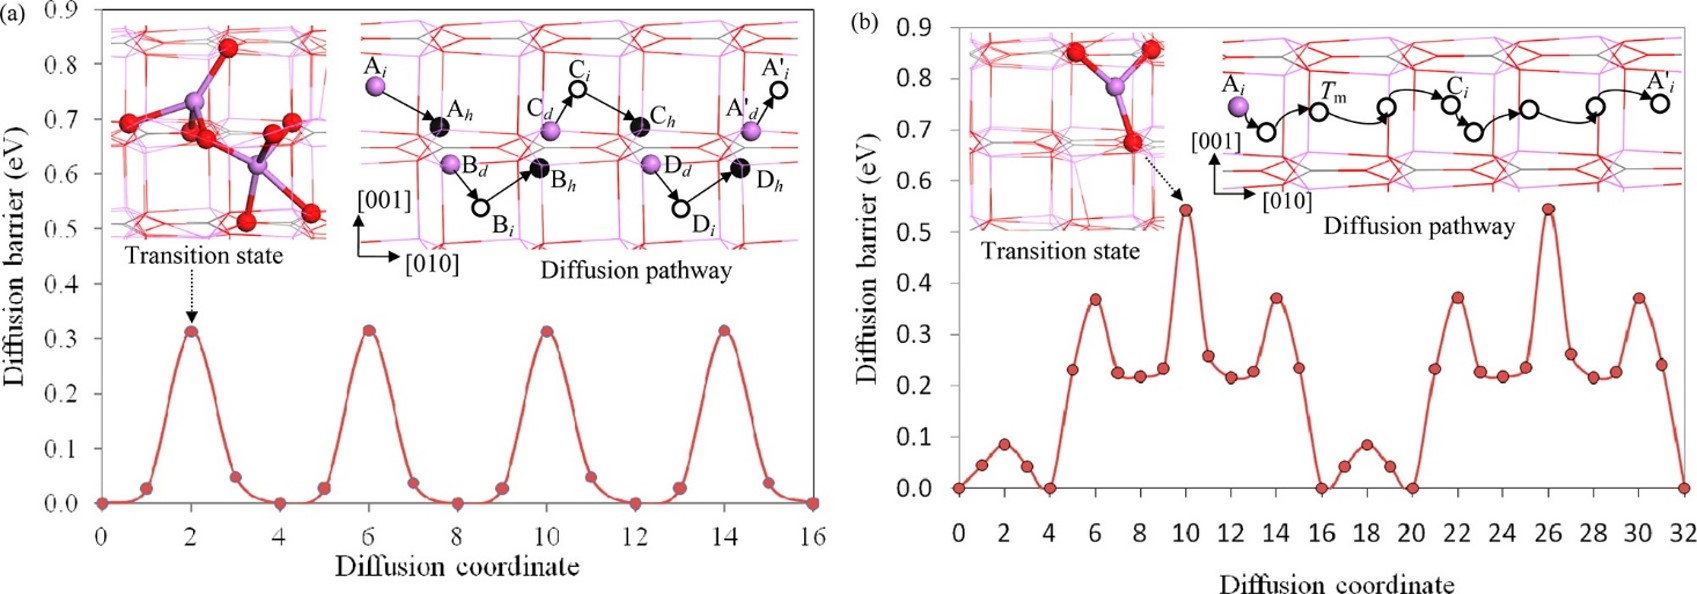
\includegraphics[scale=0.5]{figures/sei.jpg}
    \caption{Energy barrier for Li-ion transport in the SEI via (a) knock-off and (b) direct hopping mechanisms. Reprinted with permission from Ref.~\citenum{Shi2012}. Copyright 2012 American Chemical Society.}
    \label{fig:sei}
\end{figure}

The predicted values of the Li-ion diffusion energy barrier by both the implicit and the explicit models described above are significantly higher than that in the bulk of graphite, which is reported to be between 0.2-0.5 eV (c.f. section~\ref{sec:anodes_ion_diffusion}).\cite{thinius2014theoretical, Hakim, persson2010} This indicates a limiting role of the SEI in determining overall kinetics of Li-ion diffusion and the overall rate-capability of Li-ion batteries.

\subsection{C/Si composities}
\label{sec:carbon_silicon}
Use of anode materials capable of electrochemically alloying with lithium could allow higher energy densities than are possible with graphite. In particular, silicon, due to its high gravimetric capacity of 4200 mAh g$^{-1}$, has achieved tremendous attention as an anode material.\cite{larcher2007recent} Si has a low electrochemical potential 0.37--0.45 V vs. Li/Li$^+$, which is only $\sim$0.27 V higher than graphite.\cite{feng-Small-2018} Si is highly abundant, cost effective and non-toxic.\cite{nitta2014high, feng-Small-2018,Wagner-JPS-2019} While pure Si anode materials are not presently viable, present day anode materials combine a small atomic fraction (typically 5-10 at \%) of silicon with graphite to boost the gravimetric capacity of the anode.\cite{asenbauer_success_2020} However, there are certain challenges in understanding the behaviour of Si and C/Si composites that are summarised in this section.

The phase diagram of lithium and silicon shows five crystalline intermetallic Zintl-like phases: Li$_{21}$Si$_{5}$, Li$_{13}$Si$_{4}$, Li$_{7}$Si$_{3}$, Li$_{12}$Si$_{7}$, and LiSi.\cite{Okamoto1990} However, LiSi is not accessible under electrochemical conditions, since it is synthesised under high pressure, and the stoichiometry of Li$_{21}$Si$_{5}$ is disputed, with a mixed Li$_{21}$Si$_{5}$/Li$_{22}$Si$_5$ phase also proposed.\cite{gruber2013} Under electrochemical conditions, metastable phases with compositions Li$_{15}$Si$_{4}$\cite{Jiang_2020} and amorphous Li$_x$Si$_y$ can be formed.\cite{Kuhn2011} It has been proposed that a different reaction pathway between these phases during lithiation and delithiation contributes to the observed charge/discharge hysteresis in lithium silicides and C/Si composites.\cite{Jiang_2020} In particular, \citeauthor{Jiang_2020} found that the crystalline phase Li$_{15}$Si$_{4}$ is accessed during lithiation, but the lattice undergoes an amorphisation process during delithiation, with the latter step being rate determining.\cite{Jiang_2020} This limits the utility of ground state DFT calculations for understanding the Li-Si system under operating battery conditions, and is therefore a challenge for multiscale modelling. 

An additional challenge is the volume expansion. Upon full lithiation, the volume of Si can expand to more than three times its original volume, which means the Si electrodes do not retain their morphology during prolonged cycling or, even worse, some particles become detached from the electrode assembly.\cite{Wang-JPS-2014,Wagner-JPS-2019,feng-Small-2018} This volume expansion/contraction during cycling also leads to severe cracking and degradation of the SEI. It is for mainly these reasons that pure Si anodes are not currently commercially viable and must be combined with graphite. Several strategies have been proposed to change the morphology to mitigate these issues, including development of different Si robust nanostructures (0D or hollow nanoparticles, 1D nanowires, 2D film-like Si, and 3D Si structures), \cite{feng-Small-2018} and the development of composites (Si/carbon composites, Si/polymer composites, Si alloys, and Si/metal oxide composites).\cite{asenbauer_success_2020} While modelling the complex nature of the degradation pathways of the Si, Si-composites and their SEIs is presently out of reach of atomistic methods, these techniques nonetheless emerge as natural tools for high-throughput screening of different promising anode materials.\cite{kirklin2013} These approaches can also tell experimentalists the most promising part of the parameter space in which to perform more extensive, time consuming, and sometimes costly characterisation.

A more comprehensive overview of the application of mesoscale models to challenging composite systems is presented by \citeauthor{franco2019}, with the volume averaging approach highlighted perhaps being particularly applicable to Si and C/Si systems.\cite{franco2019} Particularly for carbon anodes in combination with Si or silicon suboxide (SiOx), collectively referred to as C/Si or C/SiO$_x$, it may presently be necessary to sacrifice some details of the atomic level description to enable these systems to be tractably modelled at either mesoscale or continuum levels. Regarding the dynamic and metastable behaviour described above, kMC would be a natural technique to bridge length scales and include different time scale dynamic events, as explained in a recent review dedicated to this technique.\cite{Gavil_n_Arriazu_2021_kmc}

\subsection{Outlook and challenges for anodes}
\label{sec:anodes_outlook}
Graphite remains the predominant anode material in most Li-ion cells, due to its suitably high capacity of 372 mAh g$^{-1}$, an operating potential close to 0 V vs. Li/Li$^{+}$, and its compatibility with liquid organic electrolytes. Alternative materials that form solid solutions with lithium (including silicides) presently do not have sufficient long term structural stability to be used as the primary anode material, requiring them to be composites with graphite. The development of graphite-based anodes has relied upon not only understanding staging formation in bulk, but also upon the development and understanding of a stable SEI and its implications of that SEI for cell longevity and (de)intercalation rate behaviour.

Advancements in developing all solid-state batteries (ASSBs) have resulted in additional research of Li metal anodes, as reviewed by \citeauthor{fang2019key},\cite{fang2019key} and \citeauthor{li2018developing}.\cite{li2018developing} In this section, we have summarised the safety and degradation challenges caused by lithium plating on graphite anodes. The use of Li metal as the anode for LiBs and ASSBs still face similar issues regarding redeposition of metallic Li as dendrites and consumption of cyclable lithium.\cite{fang2019key,li2018developing}

Many aspects of modelling the bulk behaviour of lithium (de)insertion graphite are well understood. As shown in this section, challenging aspects like quantifying the Li ion ordering with lithiation fraction can only be obtained by combining experimental observations with atomistic models. However, there are challenges with atomistic modelling in anodes that hinder improvements in capacity, rate performance, safety and durability of the anode itself and, consequently, full Li-ion cells. In addition, there are challenges with transferring insights from atomistic modelling in a scalable form to models on different length and time scales, while maintaining physical integrity. These outstanding challenges are:

\begin{itemize}
    \item The role of metastable phases in the kinetics of staging behaviour. New theoretical frameworks should be developed to understand the connectivity between different phases and the effect of this on the path dependency of measurable behaviour like the OCV. These distinct pathways also have implications for mechanical degradation and fracture. A promising approach in this direction is the semi-grand canonical framework developed by \citeauthor{VanderVen2020,vanderven2018} describing layered transitions in cathodes \cite{VanderVen2020,radin_role_2017,Vinck2016,vanderven2018} that could also be applicable to graphite anodes and other candidate materials like silicides. 
    \item The role of the configurational, vibrational and electronic entropy of lithium insertion. Longer length scales, i.e. continuum models, still assume that the entropy follows an ideal solid solution behaviour. The importance of configurational entropy to the phase transitions of lithium in graphite was highlighted in previous sections \cite{Mercer2019,Mercer2021,REYNIER2003850}. One promising extension would be to use the results from MC calculations to parameterise a phase field model, such as those developed by \citeauthor{Bazant2017},\cite{Bazant2017} \citeauthor{guo2016}\cite{guo2016} and \citeauthor{peng2011},\cite{peng2011} with a more realistic Hamiltonian and thus include entropy effects in a rigorous way.
    \item Regarding dynamics, kMC approaches with an empirical Hamiltonian show promise,\cite{gavilan-arriazu_kinetic_2020,gavilan-arriazu_effect_2020,GAVILANARRIAZU2018133,Gavil_n_Arriazu_2021_kmc} but are limited by the length and time scale of the properties that can currently be modelled. A possible solution would be to develop an effective cluster interaction Hamiltonian linking with a linear scaling DFT code, such as \textsc{onetep}. Parellelisation of the kMC calculations could be achieved by exploiting recently developed graphical processing unit (GPU) architectures.
\end{itemize}

Superior models of surface and interface effects are needed. This includes development of a physically rigorous version of the Butler-Volmer equation, which is valid for electron transfer but is conventionally assumed to be valid too for ionic transfer in Li-ion batteries. The current models of the interface are too simplistic or represent an ideal situation instead of dealing with the complex reality of the SEI. A systematic coarse-graining approach involving multi-length- and multi-time-scale physics can help in understanding the complex nature of the SEI and its influence on performance of Li-ion batteries. Controlling and improving the properties of SEI is crucial to improve the overall rate capability of Li-ion batteries, as that interface is the bottleneck for Li-ion diffusion.

Regarding graphite, atomistic modelling can be used to predict systematic modifications to the edge morphology or the use of dopants on the graphite edge, \cite{peng2020lithium,weydanz1994behavior,way1994effect} or tuning of the interlayer carbon spacing\cite{JI201866} to enable systematic tuning of the rate performance. This approach has the potential to lead to more robust interfaces and strategies to tune the anode voltage and dynamics, thus tuning nucleation barriers and mitigating the risk of lithium plating.\cite{peng2021} In this regard, it should be pointed out that decoupling the rate performance of different graphite edges is still a great challenge from experiment and therefore this finding represents a success for atomistic modelling.

% This part will be integrated with the new section above and summarised.
We highlight that there are still outstanding challenges regarding modelling metastable behaviour, volume expansion and degradation in solid solution materials such as silicides. So far, high-throughput atomistic modelling techniques have provided a predictive tool to suggest anode materials that are promising for more extensive experimental characterisation. However, composite materials such as C/Si and C/SiO$_x$, which are increasingly being used in commercial anodes, are presently challenging to model on the atomistic scale. In this regard, an extension to mesoscale modelling, such as a volume averaged approach as suggested by \citeauthor{franco2019}, could be a promising way to model challenging materials such as composites, in which each component experiences different degrees of volume expansion.\cite{franco2019}

\end{document}